\chapter{Implementation}
\label{chap:impl}

In this chapter, the thoughts made beforehand are outlined.
The following sections describe accurately the implementation, its components and the subsequent evaluation pipeline for disparity maps.
Chapter \ref{chap:related} pointed out that no real algorithm for stereoscopic video disparity exist yet.
For stereoscopic videos no evaluation engine yet exists.
Datasets with high-resolution stereo videos are rarely spread.
Source code for existing disparity algorithms are open-sourced and available for the public domain only in a few cases.
Additionally, there exist a lot of different unaligned code for evaluation and comparing disparity maps.
Thus, the decision towards a new implementation of an evaluation suite, built on top of OpenCV, was made.
Found source code of disparity algorithms was refloated and integrated.
Different masks for fine-grained evaluation were implemented as well.
An image diminisher which alters stereo images by adding noise, to simulate real scenery, or artifacts from video compression.
To round the evaluation suite up, a small web viewer to visualize the results was created.

\section{Preliminaries}

As development platform a MacBookPro was used with the following specifications: i5-4258U CPU @ 2.40GHz (dual-core), 8 GB RAM, a fast SSD.
For the later evaluation phase a desktop computer with an i5-2500k @ 3.30GHz (quad-core) was considered.
The programming part was done with Atom\footnote{\url{https://atom.io}}, a modern text editor, and CLion\footnote{\url{https://www.jetbrains.com/clion/}} from JetBrains, a cross-platform IDE especially for C++.
CMake as a cross-compiling makefile generator was utilized.
Everything except the web result viewer was implemented using C++.
As a timer saver and for reducing code duplicates OpenCV as master library was used.
The final build-chain consists of some shell scripts and CMake as makefile generator.
With CMake it was possible to cross-compile the app for Linux and use a fast server-instance from DigitalOcean\footnote{\url{https://www.digitalocean.com}} for the generation of the disparity maps and to actually evaluate those.
To not rely on different environments, a docker\footnote{\url{https://github.com/benjohnde/dockerbase-opencv}} image was created, open-sourced and used.
Docker helps developers to build, ship and run distributed applications.
A docker image serves as basis for containerized virtual environments.
Those docker containers work in a chroot\footnote{Chroot stands for "change root" and helps to change the root directory for a current process.} environment and are isolated from other processes.
It is not a complete virtualized machine as it runs on the system's kernel.
Some python scripts were written for the upcoming evaluation to combine all components in a chain.

\section{Overview}

Initially, a rapid monolithic prototype was built, featuring the execution of different disparity algorithms for each frame, the creation of masks and the evaluation of a given scene with different quality metrics.
But as more datasets were found and various masks as an evaluation method were established, the need for a leaner process chain arose.
Especially as disparity algorithms need some time to compute the disparity map for one frame.
Hence, as videos consist of multiple frames (in our datasets about 100 frames in mean) this is a time consuming task.
Sometimes metrics change, the threshold is adjusted or a new metric is found.
\newline\newline\noindent As a result, an approach towards small services with which computed disparity maps can be evaluated repeatedly and independently.
Thus, the monolithic prototype was rewritten and partitioned in smaller microservices shaping three different components:

\begin{itemize}
  \item disparity algorithm executer,
  \item mask creator,
  \item evaluation engine.
\end{itemize}

\noindent Additionally, a small tool for diminishing images was created.
It can simulate real scenery by adding gaussian noise as recommended by \citep{richardt2010real}.
In addition, FFmpeg \citep{FFMPEG2010} was wrapped to simulate artifacts originating from video compression.
The output, which each one of those microservices in the chain can generate or operate on, is structured in a simple folder tree.
\newline\newline\noindent The Figure \ref{fig:impl-pipeline} shows the composition and the evaluation chain of these microservices.

\tikzstyle{rblock} = [text width=10em, rectangle, draw, fill=blue!20, text centered, rounded corners, minimum height=4em]
\tikzstyle{cloud} = [text width=6em, ellipse, draw, fill=red!15, text centered, rounded corners, minimum height=3.2em]
\begin{figure}[hp!]
  \centering
  \begin{tikzpicture}[node distance=7em, auto]
    %input
    \node [cloud] (right) {right image};
    \node [cloud, right of=right, node distance=10em] (left) {left image};
    \node [cloud, right of=left, node distance=10em] (disp) {ground-truth};

    %computation
    \node [rblock, below of=right, xshift=2em] (exec) {(1) Algorithm executer};
    \node [rblock, below of=disp, xshift=-2em] (mask-creator) {(2) Mask creator};

    %output
    \node [cloud, below of=exec] (map) {disparity map};
    \node [cloud, below of=mask-creator] (masks) {masks};

    %evaluation
    \node [rblock, below of=left, yshift=-14em] (evaluation) {(3) Disparity evaluator};

    %final result
    \node [cloud, below of=evaluation, xshift=-5em] (csv) {CSV file};
    \node [cloud, below of=evaluation, xshift=5em] (heatmaps) {heatmaps};

    %lines
    \path [line] (right) -- (exec);
    \path [line] (left) -- (exec);
    \path [line] (left) -- (mask-creator);
    \path [line] (disp) -- (mask-creator);

    \path [line] (exec) -- (map);
    \path [line] (mask-creator) -- (masks);

    \path [line] (map) -- (evaluation);
    \path [line] (masks) -- (evaluation);

    \path [line] (evaluation) -- (csv);
    \path [line] (evaluation) -- (heatmaps);
  \end{tikzpicture}
  \caption{Composition and processing pipeline of the implementation.}
  \label{fig:impl-pipeline}
\end{figure}

\section{Evaluation engine for videos}

In contrast to other implementations, input and output are clearly defined and thus different techniques can be adapted easily.
There exist combined frameworks which fulfill two tasks, disparity calculation (as the algorithm is implemented) and the final evaluation step.
This makes it harder to use the evaluation module separately from the rest.
None the less the open source community around computer vision also lacks of code for stereo matcher.
Due the diversities of algorithms and eval suites the decision was made to go for an OpenCV implementation of an eval suite for disparity algorithms.
\newline\newline\noindent At the current point in time, no disparity algorithms that directly target videos yet exist.
As a video is defined by multiple consecutive frames, every disparity algorithm for images can also be applied on videos.
The drawback of this trivial approach is the lack of taking the correlation of the frames into account.
None the less it is possible to focus on some other details.
\newline\newline\noindent For instance, possible outliers in the sense of frames can occur, which may lead to more erroneous results.
The mean performance (error rate) of algorithms on a complete scene can be analyzed.
The runtime may vary in a sequence from frame-to-frame.
It is also interesting to see the impact of image diminishing effects like compression or noise, simulated as occurring from converting the signal from a real sensor.
This is more described in the upcoming section regarding image diminishing effects.
\newline\newline\noindent As middleware between the components OpenEXR\footnote{\url{http://www.openexr.com}} is used.
OpenEXR is a file format for high dynamic-range (HDR) images.
It supports 32-bit floating-point values and is thus good for representing sub-pixel accurate values in a disparity map.
The file format is also integrated in OpenCV yet.
For the later evaluation, the comparison of ground-truth data with computed disparity maps, the file format is sufficient.
However, for visualization the values have to be normalized in a range suitable for using sophisticated color ranges like RGB.
Hence, heatmaps are created with normalized disparity maps in the range of $0-255$.
\newline\newline\noindent Basically, the evaluation engine needs a computed disparity map and the ground-truth counterpart.
Only comparing both provides low informative value.
Algorithms tend to produce disparity maps with a few unknown fields (e.g. occluded pixels).
Crucial are also depth-discontinuity along object borders, textureless regions and occluded pixels.
Thus, masks are used to only focus on these particular areas.
The creation of these masks are illustrated accurately in the upcoming section.
The masks are used in combination with quality metrics, which are introduced in Chapter \ref{chap:eval}, in which evaluation and results are discussed.
The evaluation engine applies these quality metrics in combination with masks and outputs the result in a simple CSV file\footnote{CSV stands for comma-separated values. A CSV file usually represents a table, with rows being the lines and in columns the values are separated with commas.}.
\newline\newline\noindent Python scripts round the evaluation engine up.
They work basically as a wrapper to iteratively execute each component over each frame of a given input sequence and aggregate the results.
The evaluation engine, as well as the other components, are run with command line arguments to pass specific parameters for the execution, for instance which input images should be used and where the computed disparity map should be saved.

\tikzstyle{rblock} = [text width=8em, rectangle, draw, fill=blue!20, text centered, rounded corners, minimum height=4em]
\tikzstyle{cloud} = [text width=6em, ellipse, draw, fill=red!15, text centered, rounded corners, minimum height=3.2em]
\begin{figure}[hp!]
  \centering
  \begin{tikzpicture}[node distance=6em, auto]
    %input
    \node [cloud] (computed) {computed disparity map};
    \node [cloud, below of=computed] (groundtruth) {ground-truth disparity map};
    \node [cloud, below of=groundtruth] (result) {CSV file};
    %computation
    \node [rblock, right of=computed, xshift=7em, yshift=-3em] (init) {init with input};
    \node [rblock, below of=init] (compare) {compare masked pixels};
    %lines
    \path [line] (computed) -- (init);
    \path [line] (groundtruth) -- (init);
    \path [line] (init) -- (compare);
    \path [line] (compare) -- (result);
  \end{tikzpicture}
  \caption{Illustration of evaluation engine.}
  \label{fig:impl-evaluation-engine}
\end{figure}

\section{Integration of existing algorithms}

%todo more text in each subsection
%todo a bit talking about parameters

The decision, which algorithm should be implemented was not an easy task as shown in the related work Chapter \ref{chap:related}.
There is a huge diversity of used technologies amongst disparity algorithms: various programming languages, cpu versus a cuda implementation, different coding styles and used libraries.
As a matter of fact, this makes it harder to implement and evaluate every available disparity algorithm.
Here a more streamlined extendable architecture is presented.
The algorithms, which were introduced in the related work Chapter \ref{chap:related}, are adopted and integrated.
The architecture of the disparity interface is depicted in Figure \ref{fig:uml-disparity-interface}.

\begin{figure}[h!]
  \centering
  \begin{tikzpicture}
    %classes
    \umlclass[x=2.5,y=8,type=abstract]{DisparityAlgorithm}{- left: cv::Mat\\- right: cv::Mat}{- compute()}
    \umlclass[x=0,y=5.3]{ELASAlgorithm}{}{}
    \umlclass[x=4.5,y=5.3]{MRFStereo}{}{}
    \umlclass[x=2.5,y=3,type=interface]{OpenCVStereoMatcher}{}{}
    \umlclass[x=0,y=0]{OpenCVStereoBM}{}{}
    \umlclass[x=5,y=0]{OpenCVStereoSGBM}{}{}
    %connections
    \umluniassoc{OpenCVStereoMatcher}{DisparityAlgorithm}
    \umluniassoc{ELASAlgorithm}{DisparityAlgorithm}
    \umluniassoc{MRFStereo}{DisparityAlgorithm}
    \umlimpl{OpenCVStereoBM}{OpenCVStereoMatcher}
    \umlimpl{OpenCVStereoSGBM}{OpenCVStereoMatcher}
  \end{tikzpicture}
  \caption{Architectural overview on the disparity interface in form of an UML diagram.}
  \label{fig:uml-disparity-interface}
\end{figure}

\noindent The abstract class \texttt{DisparityAlgorithm} provides both images, left and right one, in form of a \texttt{cv::Mat} object.
On top of this abstract class further algorithms can be adopted easily.
The output of each algorithm is then streamlined and put in the destination file.

\subsection*{OpenCV}

OpenCV offers two algorithms, simple block matching and the semi-global block matcher based on the implementation of \citeauthor{hirschmuller2008stereo}.

\subsection*{Middlebury MRF library}

The Middlebury MRF library \citep{scharstein2006middlebury} consist of three parts, which all have to be composed together:
\begin{itemize}
  \item The imageLib, a small library for 2D multi-band images.
  \item MRF, an energy minimization software \citep{szeliski2008comparative}.
  \item mrfstereo, which is a stereo matcher front-end for the MRF library.
\end{itemize}

\noindent Some patches need to be applied to the MRF energy minimization software in order to get the graph cuts algorithms to work.
The composition is open-sourced\footnote{\url{https://github.com/benjohnde/disparity-algorithms}} with a Makefile.
Finally, a small wrapper for the execution was created.

\subsection*{ELAS: Efficient large-scaler stereo matching}

ELAS is integrated, like the Middlebury MRF library, with a simple wrapper which executes the ELAS binary.
ELAS required the input files as PGM\footnote{PGM is a grayscale image format, part of the Netpbm library.} and outputs PFM\footnote{Similar to OpenEXR, PFM is a floating-point image file format, also part of the Netpbm library.} images.
In a preprocessing step the input stereo images are temporarily saved in the PGM format as grayscale.
After the execution of ELAS, as a postprocessing step, the PFM files are converted to OpenEXR files, as the subsequent processes expect OpenEXR files as input.
For processing the PFM files, a simple file reader was created, according to the official specifications\footnote{\url{http://netpbm.sourceforge.net/doc/pfm.html}}.
Specific characteristics of this file format are that the rows are written bottom-to-top and each column has to be multiplied with a so called scale factor.

\section{Fine-grained evaluation via masks}

The evaluation would be trivial by just comparing the computed disparity map with its ground-truth companion.
This trivial comparison would be a pitfall, as the results would be erroneous due to a variety of reasons.
To give an example, occluded regions would lead to a higher error rate.
As remedy, masks are introduced to simply focus on interesting pixels.
Masks are normal matrices of the size of the input image and they reflect two states $0$ and $1$ like a bit, whereas $1$ stands for masked.
In the literature they sometimes also named bitmasks.
In this section the following masks are introduced and how they are determined:

\begin{itemize}
  \item depth-discontinuity,
  \item textured regions,
  \item occluded pixels,
  \item salient regions.
\end{itemize}

\noindent Programmatically they are represented through the OpenCV matrix class \texttt{cv::Mat} which can not work as a binary matrix and obtain just two states.
Thus, a \texttt{cv::Mat} with \texttt{CV\_8U1} is initialized, which means one color channel utilizing 8-bit unsigned for the values.
In this matrix, $255$ represents a $1$.

\subsection*{Depth-discontinuity}

Determining correspondence can fail in textureless or depth-discontinuous regions as mentioned beforehand in Chapter \ref{chap:foundations}.
Thus, it is interesting to see how disparity algorithms handle such regions.
So, a depth-discontinuity mask was implemented.
Depth-discontinuity is observed in the ground-truth disparity map.
It is defined as regions, where adjacent disparities differ by more than a certain gap \citep{scharstein2002taxonomy, cyganek2011introduction}.
For this purpose two basic morphological\footnote{Morphological operations are techniques to analyze and process geometrical structures.} image processing operations from the OpenCV library are used: \texttt{dilate} and \texttt{erode}.
\texttt{dilate} outputs for each position in a \texttt{cv::Mat} the maximum value of all the pixels in the neighborhood.
\texttt{erode} does nearly the same, but returns the minimum value.
Both are fed with a kernel, specifying which adjacent pixels should be taken into account.
\newline\newline\noindent For getting the disparity gap, the image gets dilated to get the maximum disparity of a pixel's neighbor.
Then eroded to estimate the minimum disparity of a pixel's neighbor.
Both is done with a $3x3$ kernel, and all adjacent pixels are masked to observe.
Finally, the depth-discontinuity areas are the ones with $maximum - truth > gap$.
The depth-discontinuity is then dilated by a window with given width to intense the area.
Visually, the best results are achieved with a gap of $2.0f$ and a width of $3$ for the final dilation.
Figure \ref{fig:dd-mask} depicts this.

\begin{figure}[h!]
\centering
\begin{tabular}{ccc}
\subfloat[ground-truth disparity]{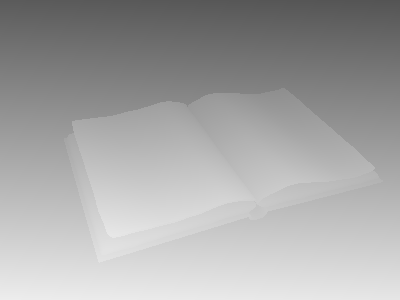
\includegraphics[width=0.3\textwidth]{src/images/book_ground-truth.png}} &
\subfloat[mask before final dilation]{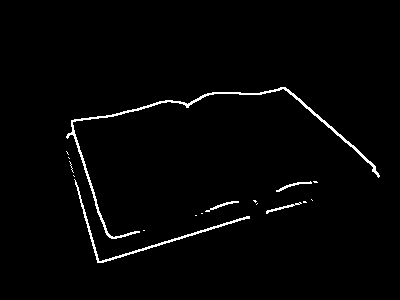
\includegraphics[width=0.3\textwidth]{src/images/book_dd_mask.png}} &
\subfloat[final mask for evaluation]{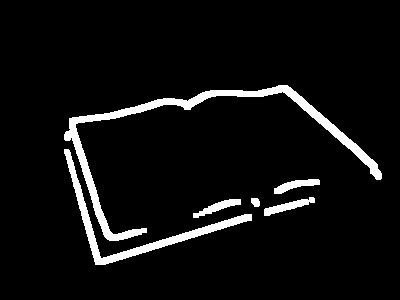
\includegraphics[width=0.3\textwidth]{src/images/book_dd_mask_final.png}}
\end{tabular}
\caption{A depth-discontinuity mask, exampled with the first frame of the book scene from the Middlebury dataset.}
\label{fig:dd-mask}
\end{figure}

\subsection*{Textured regions recognition}

Stereo matching algorithms act on the assumption, that disparity is smooth, especially if contrast and color intensity do not change drastically.
Therefore, it can be interesting to see how those algorithms treat textured and textureless regions.
Basically, regions with little or no texture in an image is defined as areas, where the squared horizontal intensity gradient, averaged over a square window of a given size, is below a given threshold \citep{scharstein2002taxonomy, cyganek2011introduction}.
This is done with the OpenCV implementation of \texttt{Sobel} and \texttt{Boxfilter}.
Figure \ref{fig:textured-mask} depicts this approach.

%todo may be a bit more on the filter and what is implemented.

\begin{figure}[h!]
\centering
\begin{tabular}{ccc}
\subfloat[image of left camera]{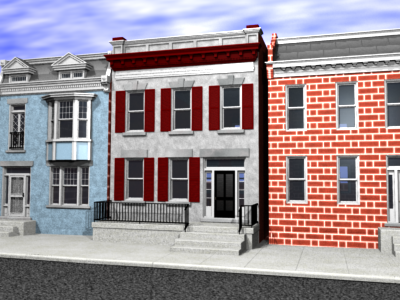
\includegraphics[width=0.4\textwidth]{src/images/street_left.png}} &
\subfloat[final textured mask]{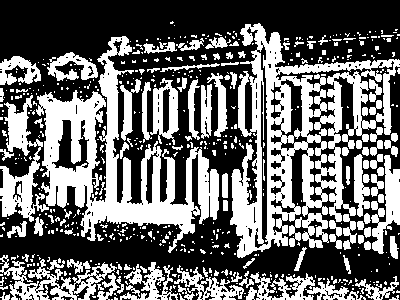
\includegraphics[width=0.4\textwidth]{src/images/street_textured_mask.png}} &
\end{tabular}
\caption{Textured regions recognition with the first frame of the street scene from the Middlebury dataset.}
\label{fig:textured-mask}
\end{figure}

\subsection*{Discover occluded pixels}

An occluded pixel is defined as a pixel, which is hidden in one of the two images, for instance an object hides it from a different angle.
In the case of stereo matching the disparity can not be calculated for such pixels
Thus, occluded pixels have to be handled properly, as they could distort our result.
For this purpose, a simple mask for non-occluded areas is introduced, to indicate which pixels on the scene are visible for both cameras and which are not.
\newline\newline\noindent To obtain the mask both disparity maps, left and right one, are iterated.
Pixels that are visible from both cameras should have the same disparity value in both disparity maps.
For occluded pixels, the value is different \citep{martull2012realistic}.
Hence, a simple cross-check is sufficient.
Figure \ref{fig:noc-mask} shows an example of such a non-occluded areas mask.

\begin{figure}[h!]
\centering
\begin{tabular}{ccc}
\subfloat[left ground-truth]{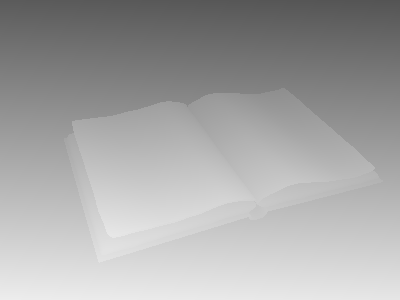
\includegraphics[width=0.3\textwidth]{src/images/book_ground-truth.png}} &
\subfloat[right ground-truth]{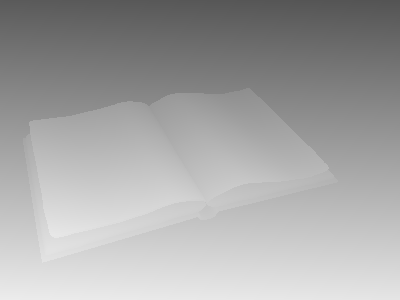
\includegraphics[width=0.3\textwidth]{src/images/book_ground-truth_right.png}} &
\subfloat[resulting mask]{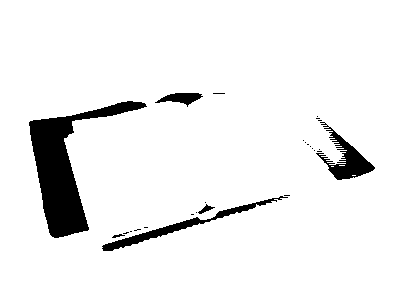
\includegraphics[width=0.3\textwidth]{src/images/book_noc_mask.png}}
\end{tabular}
\caption{The ground-truth disparity maps of the first frame of the book scene from the Middlebury dataset is used to illustrate the non-occluded areas mask.}
\label{fig:dd-mask}
\end{figure}

\subsection*{Saliency detection}

As a novel approach, saliency detection is used is another criteria for the later evaluation.
It is interesting to see how disparity algorithms operate on salient regions in an image.
There exist some algorithms for saliency detection in images and videos \citep{dittrich2013saliency, hou2007saliency, opencv_library}.
OpenCV offers two different saliency detection algorithms:
\begin{itemize}
  \item \texttt{StaticSaliency} in images, and
  \item \texttt{MotionSaliency} on videos.
\end{itemize}

\noindent Here the static saliency approach was used \citep{hou2007saliency}.

%todo a bit more how it was implemented and what the basic idea behind this saliency detection is

\section{Image diminisher to simulate real use cases}

It is also interesting to see the impact of image diminishing effects like compression or noise like from a real sensor.
Both can be simulated.
Noise can be added onto the rendered video.
Then the impact can be analyzed.
Video compression is added via FFmpeg.

%todo impl flow of diminisher

\subsection*{Gaussian noise}

As seen in the related work Chapter \ref{chap:related}, some approaches use restoration algorithms in order to reduce noise which can occur.
Hence, noise generation was added as a preprocessing step in order to see how noise disrupts disparity algorithms.
Gaussian noise is used, meaning that the noise is gaussian distributed (or normal distributed).
\newline\newline\noindent $\mu$ is the mean value (= 0).
$\sigma$ is the standard deviation.
Normal (gaussian) distribution is denoted as $\mathcal{N}(\mu,\sigma^2)$, where $\mu$ is the mean and $\sigma^2$ the variance.
\newline\newline\noindent The variance, $\sigma^2$ can be set in our evaluation suite in order to see how this distracts the image.
As recommended by \citep{richardt2010real}, gaussian noise is added to synthetic video sequences with a mean of $20$ to simulate real scenery.
The distribution is illustrated in Figure \ref{fig:gaussian}.

\pgfmathdeclarefunction{gauss}{2}{%
  \pgfmathparse{1/(#2*sqrt(2*pi))*exp(-((x-#1)^2)/(2*#2^2))}%
}
\begin{figure}[h!]
  \center
  \begin{tikzpicture}
    \begin{axis}[every axis plot post/.append style={
      mark=none,domain=17:23,samples=50,smooth}, % All plots: from -2:2, 50 samples, smooth, no marks
      axis x line*=bottom, % no box around the plot, only x and y axis
      axis y line*=left, % the * suppresses the arrow tips
      enlargelimits=upper] % extend the axes a bit to the right and top
      \addplot {gauss(20,0.6)};
      \addplot {gauss(20,0.8)};
      \addplot {gauss(20,1.0)};
    \end{axis}
  \end{tikzpicture}
  \label{fig:gaussian}
  \caption{Gaussian noise distribution with $\mathcal{N}(20,\sigma^2)$ and different values for $\sigma^2$.}
\end{figure}

\noindent It is added with the \texttt{randn}\footnote{\url{http://docs.opencv.org/master/d2/de8/group__core__array.html\#gaeff1f61e972d133a04ce3a5f81cf6808}} function of the OpenCV library \citep{opencv_library}.
It generates a \texttt{cv::Mat} with the random distribution of values.
This matrix is then added on the source matrix, resulting in a noisy image.
Salt and pepper noise was not chosen, as it does not reflect real scenery.
Salt and pepper noise is not a common noise, as it contains random occurrences of black and white pixels.
It mostly appears by defect image sensors or erroneous analog-to-digital conversion.

\subsection*{Video compression}

Most of the widely used video compression techniques belong to the lossy data compression algorithms.
As in contrast to lossless compression, lossy tend to produce small artifacts in images or videos as it does not reconstruct the original data as a whole.
FFmpeg \citep{FFMPEG2010} is used to simulate the degradation of stereo videos.
FFmpeg is a tool to create video sequences from images with popular video codecs and also to divide a video sequences into images.
\newline\newline\noindent Bla.
%todo how it is implemented what codec is used mainly?
%todo impl flow of ffmpeg

\section{Web result viewer for evaluation suite}

For fine-tuning the algorithm's parameters as well as implementing the bitmasks it was helpful to see the visual output of both.
As the resulting bitmasks for each frame with the computed result disparity map were saved on the hard-drive for further investigations a web result viewer was created for visualizing the output.
The following features were implemented:
\begin{itemize}
  \item Starting new computations with different parameters and scene selection.
  \item Playing frame-by-frame with different speeds.
  \item Online csv-export of result.
\end{itemize}

\begin{figure}[p!]
  \centering
  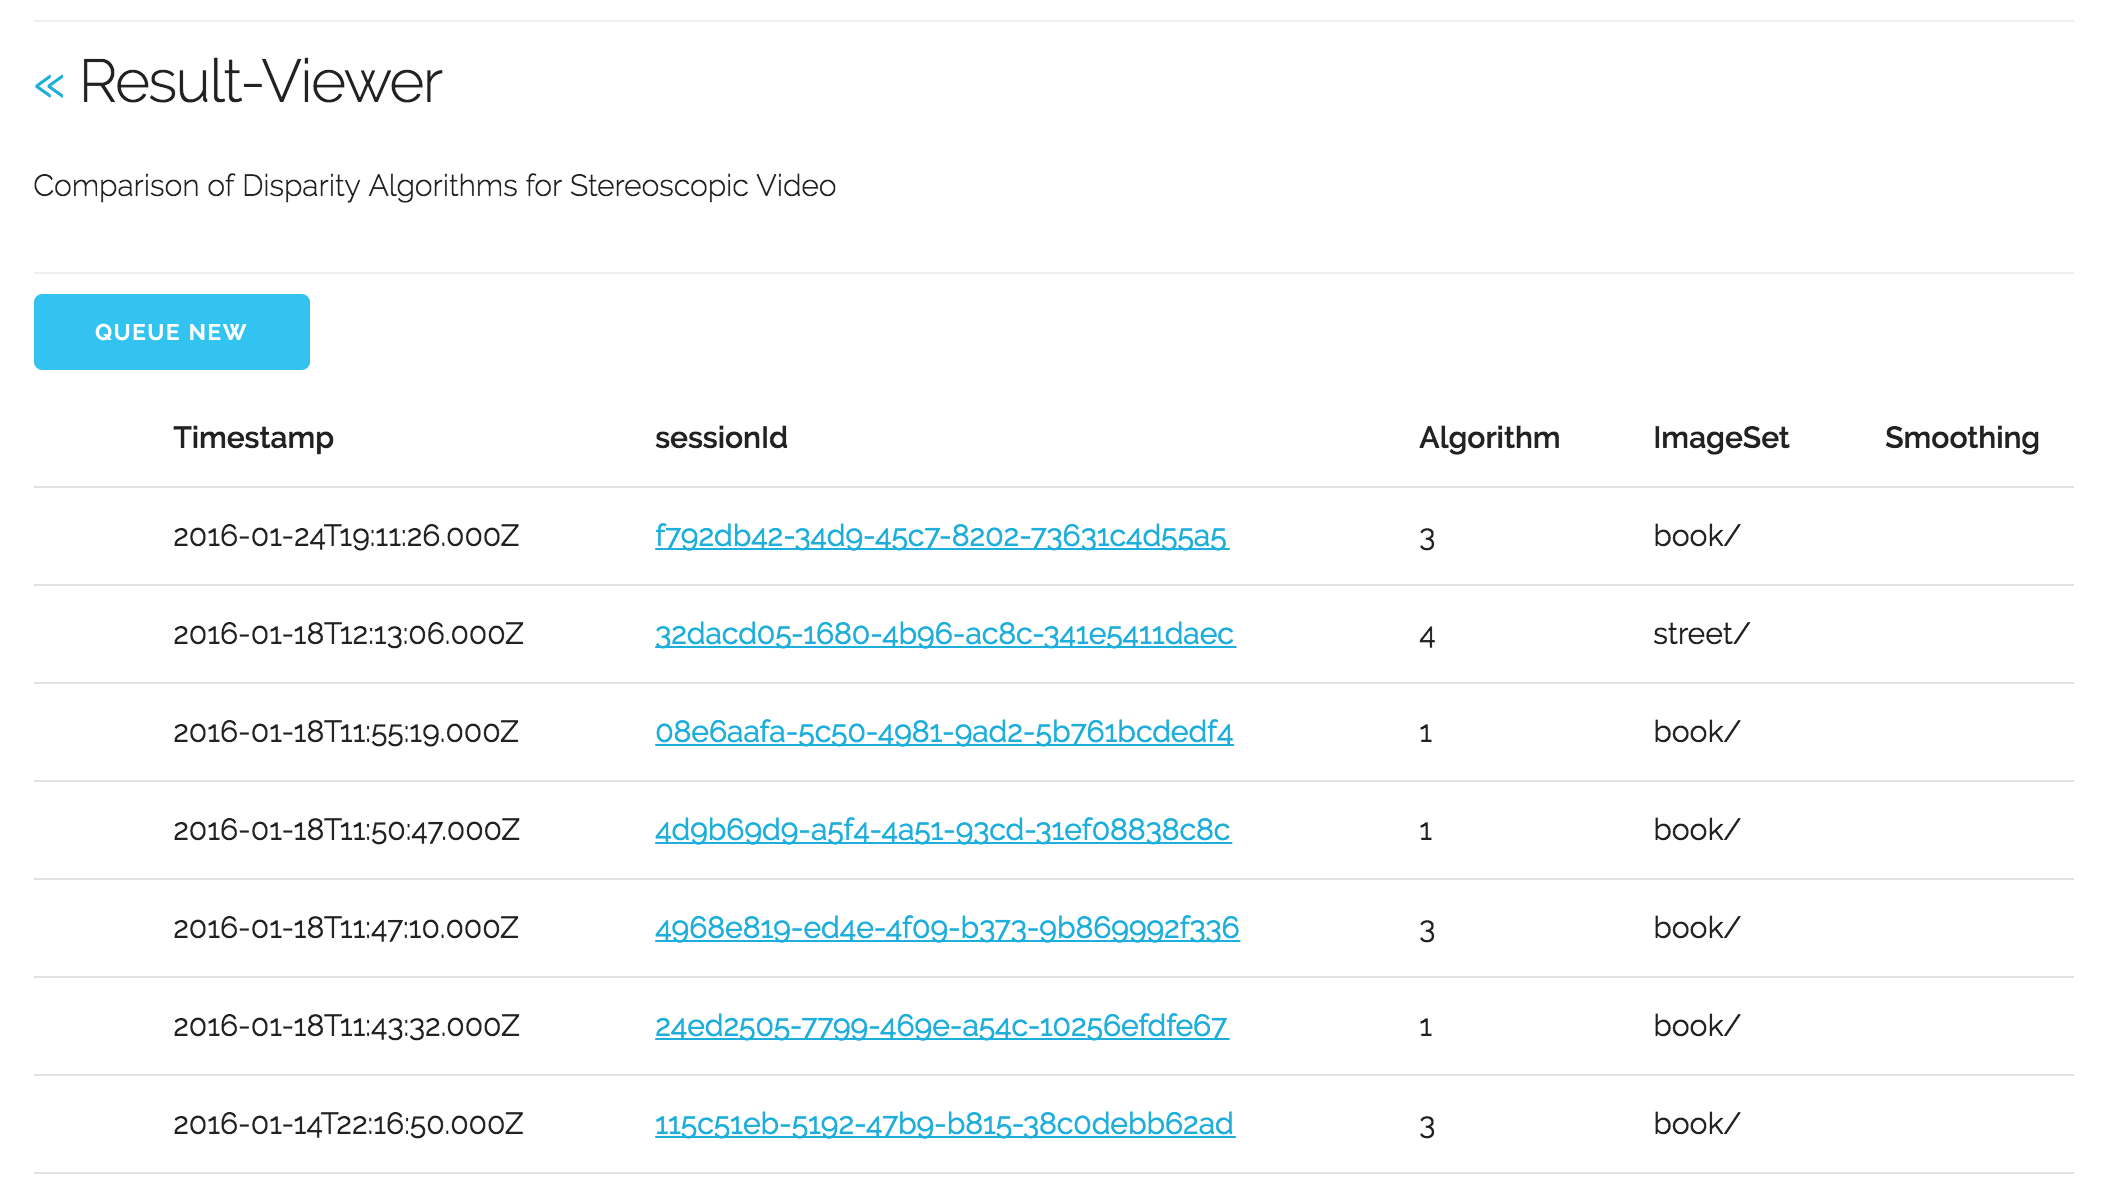
\includegraphics[angle=90,width=0.7\textwidth]{src/images/result-viewer-overview.png}
  \caption{Overview page of web result viewer.}
  \label{fig:web-overview}
\end{figure}

\begin{figure}[p!]
  \centering
  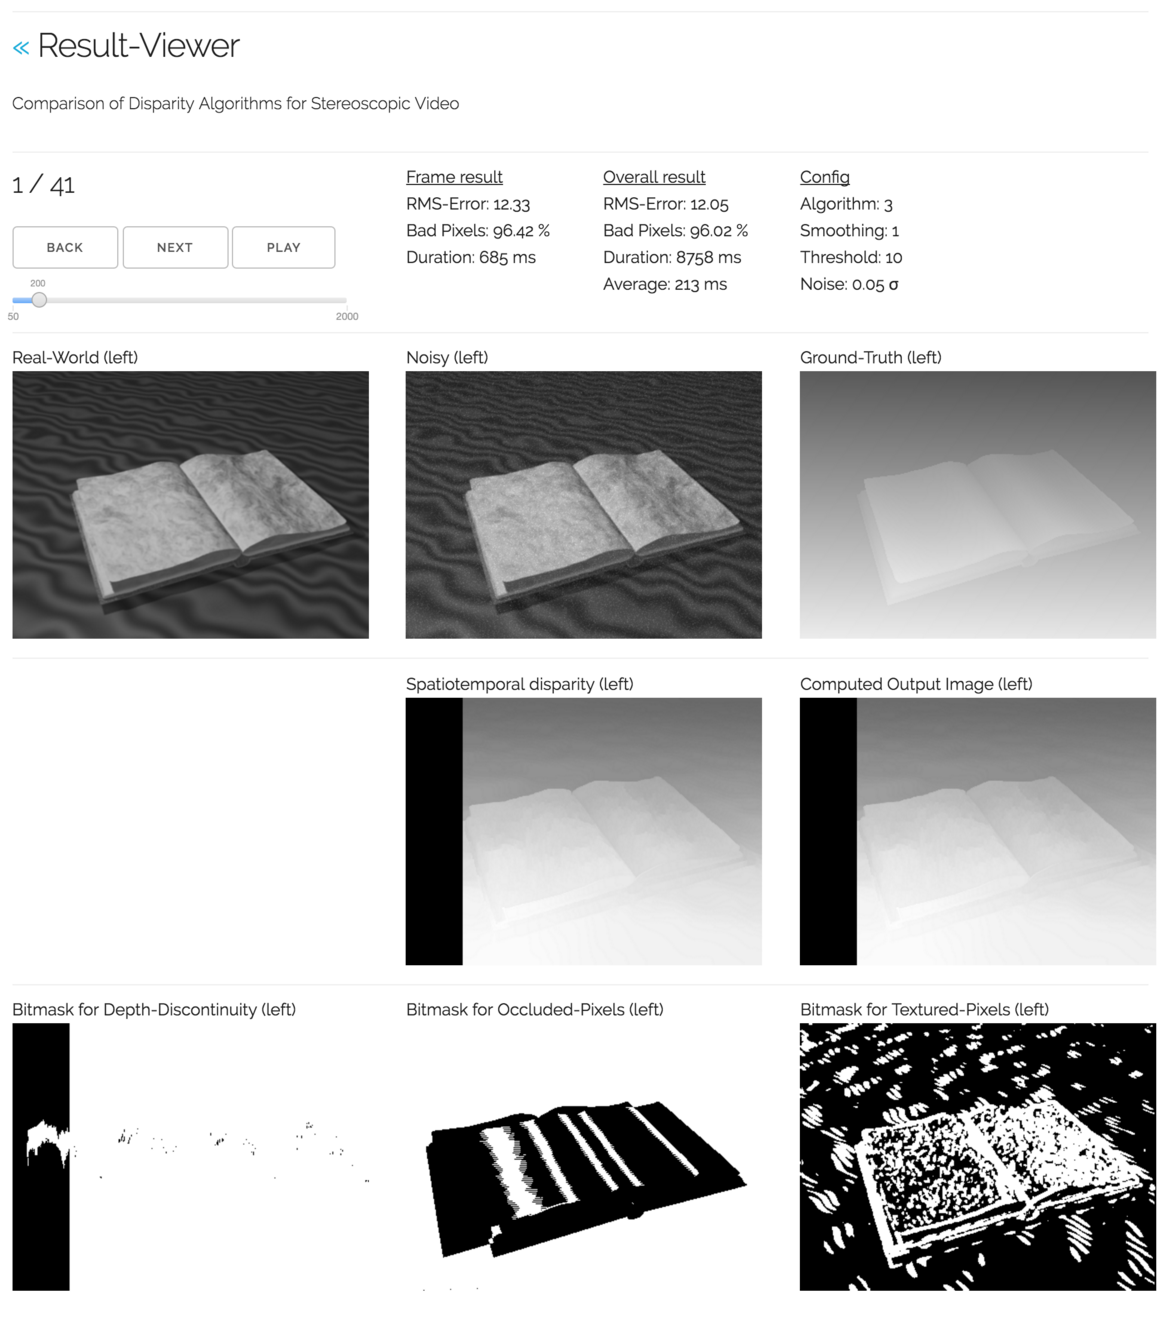
\includegraphics[angle=90,width=1.0\textwidth]{src/images/result-viewer-detail.png}
  \caption{Detail of one result in the web result viewer.}
  \label{fig:web-detail}
\end{figure}

%todo finish web result viewer section
\begin{itemize}
  \item Insert screenshot (one or two from web result viewer)
  \item Describe basic features
  \item Describe what could be done with the evaluation web suite in near future
  \item But for thesis evaluation a csv exporter was used.
\end{itemize}

\section{Discussion}

%todo summarize a bit

The following modules were actually implemented:

\begin{itemize}
  \item Reader for the PFM file format.
  \item Python scripts for upcoming evaluation.
  \item Shell scripts for getting the docker containers and thus the work distributed among different instances\footnote{With instances virtual machines from DigitalOcean are meant.}.
  \item Evaluation processor for
\end{itemize}
